\chapter[CADRE CONCEPTUEL ET THÉORIQUE]{CADRE CONCEPTUEL ET THÉORIQUE}    
    \section{Introduction partielle}
    Actuellement, l’informatique est devenue l’outil privilégié de l’information dans
    différentes entreprises. D’où sa nécessité s’impose dans tous les domaines de gestion et la
    maitrise de l’outil informatique qui constitue la garantie d’une bonne gestion, d’un bon
    fonctionnement et donc une bonne rentabilité de cette dernière.
    \section[Cadre Conceptuel]{Cadre conceptuel}
    Le cadre conceptuel met en relation les concepts
    fondamentaux du travail de recherche. Dans cette
    section, nous allons aborder les théories existantes
    relatives à notre domaine d’étude comprenant trois
    aspects à savoir :
    \par
        \begin{enumerate}
            \setlength{\itemsep}{0pt}
            \item La gestion de la relation client
            \item La fidélisation de la clientèle
            \item Les outils d’écoute
            \item Le système décisionnel
        \end{enumerate} 
        \subsection[La gestion de la relation client]{La gestion de la relation client}
            La gestion de la relation client (CRM, customer
            relationship management en anglais) est la capacité
            à bâtir une relation profitable sur le long terme
            avec les meilleurs clients en capitalisant sur 
            l’ensemble des points de contacts par une allocation optimale
            des ressources. \cite*{Lefebure2005}
            \par
            L’objectif de la gestion de la relation client
            est de créer et d’entretenir une relation réciproquement
            bénéfique entre l’entreprise et ses clients.
        \subsection[La fidélisation de la clientèle]{La fidélisation de la clientèle}
            La fidélisation de la clientèle consiste à mettre
            en place des actions marketing et commerciales
            pour construire une relation durable avec les
            clients et les inciter à renouveler leurs achats
            dans un laps de temps plus ou moins long. \cite*{Maud2022}
            \par
            Cela peut inclure des programmes de fidélité, des offres
            spéciales, des récompenses, etc.
            L’objectif est de créer un attachement à la marque et
            d’encourager les clients à revenir.
            \par
            Les entreprises qui parviennent à bien cerner ce qu’est
            la fidélisation de la clientèle et son importance n’hésitent
            pas à mener toutes les actions possibles pour rendre les clients
            fidèles, car en capitalisant sur les clients satisfaits
            qui achètent et consomment les produits et services, les entreprises
            peuvent générer des revenus réguliers. \cite*{Maud2022}
            % La fidélisation est considérée comme un concept
            % marketing qui touche aussi le domaine de la relation client
            %
            % Même si la fidélisation représente davantage un concept marketing,
            %elle concerne également le domaine de la relation client.
            \subsubsection[Enjeux de la fidélisation]{Enjeux de la fidélisation}
            Sur des marchés de plus en plus saturés,
            où la situation concurrentielle se durcit, il apparait que les coûts de prospection
            de nouveaux clients sont supérieurs aux coûts de conservation des clients. \cite*{Reichheld2001loyalty}
            De ce fait, une société rationnelle préfère investir pour conserver
            les clients qu’il a, plutôt que de tenter de conquérir les clients servis par
            la concurrence.
            \par
            Des études montrent qu’il existe en longue période une corrélation entre capacité
            d’une organisation à fidéliser ses clients (taux de rétention élevé) et ses
            résultats concrets (exprimés en part de marché, en rentabilité et en croissance). \cite*{Reichheld2001loyalty}
            %% A MODIFIER
            Les entreprises qui sont en
            mesure de conserver leur base clientèle et en particulier leurs « bons clients »
            sont celles qui non seulement résistent le mieux aux dépressions conjoncturelles,
            mais aussi sont les plus capables de financer leurs projets de développement.
        \subsection[Les outils d’écoute]{Les outils d’écoute}
        La perception que l’on a de sa clientèle est subjective et partielle.
        Les outils de la satisfaction du client sont des analyseurs plus objectifs de la clientèle, 
        et parviennent à favoriser l’amélioration de la qualité des prestations et de la satisfaction du
        client.
            \subsubsection[Évaluer la satisfaction]{Évaluer la satisfaction}
            L’évaluation de la satisfaction est réalisée après chaque prestation ou après une période
            bien définie au cours de l’année, auprès d’un échantillon de la clientèle. Cette évaluation doit être effectuée, car les organisations ont plutôt
            tendance à se cacher les insatisfactions de leurs clients pour différentes raisons :
            \par    
                \begin{itemize}
                    \setlength{\itemsep}{0pt}
                    \item [\ding{226}] Par appréhension du jugement des clients,
                    \item [\ding{226}] Pour éviter d’éventuels conflits qui pourraient
                    résulter de la révélation des insatisfactions,
                    \item [\ding{226}] Pour ne pas se sentir dévalorisées.
                \end{itemize}
            Le but de l’évaluation de la satisfaction est donc : de recueillir l’avis des
            clients sur les prestations et les produits délivrés par la société,
            de repérer les sources d’insatisfaction, de réduire les insatisfactions que l’on juge
            préjudiciables à la bonne marche des activités de la société, d’améliorer ainsi
            l’image et la compétitivité de l’activité de la société. \cite*{Barouch2010}
            \par
            Pour une évaluation, simplifiée, de la satisfaction on lance généralement
            une enquête suivant les étapes définies comme vu dans
            \cite[Tab. \ref{table:etapeDeRealistaionEnqSatisfat}]{Barouch2010} :
            %     $$\overline {x}=\sum_{i=1}^{n} w_{i} x_{i} \mathbin{/} \sum_{i=1}^{n} w_{i}$$
            \begin{longtable}{p{2cm} p{5cm} p{6cm}}
                \caption{Étapes de réalisation d’une enquête de satisfaction}
                \label{table:etapeDeRealistaionEnqSatisfat}
                \\\hline\hline
                    \textbf{Étapes} & \textbf{Action à réaliser} & \textbf{Point cl{\'e}s}
                \\\hline\hline
                    1 & Définir la liste des clients à interroger.
                    & Interroger tous les clients ou bien un échantillon de la clientèle.
                    \\
                    2 & Définir le contenu du questionnaire & Établir
                    un questionnaire simplifié ou questionnaire développé
                    \\
                    3 & Faire passer le questionnaire & Créer la motivation à répondre
                    \\
                    4 & Réaliser la synthèse des résultats & Calculer la moyenne des notes
                    obtenues
                    \\
                    5 & Définir les actions d’amélioration & Analyser et compenser les points
                    faibles 
                \\\bottomrule
            \end{longtable}
            \subsubsection[Les indicateurs de suivi de la clientèles]{Les indicateurs de suivi de la clientèle}
            Le client fait vivre le professionnel et justifie son activité.
            La qualité de la relation client a un effet direct sur ses résultats économiques.
            Les indicateurs de suivi de la clientèle permettent d’évaluer de façon
            objective dans quelle mesure le professionnel satisfait les besoins
            de sa clientèle. La progression de ces indicateurs donne donc une base solide à l’activité.
            \par
            Nous retrouvons trois types d’indicateurs :
            \par
            \begin{itemize}
                \setlength{\itemsep}{0pt}
                \item [\ding{226}] \textbf{Les indicateurs de satisfaction} :
                Un indicateur de satisfaction est un outil utilisé pour mesurer
                la satisfaction des clients envers un produit, un service ou une
                entreprise. Il existe plusieurs indicateurs pour mesurer la
                satisfaction client, tels que le nombre de réclamations ou
                les indices de satisfaction des clients.
                \item [\ding{226}] \textbf{Les indicateurs de fidélisation} :
                un indicateur de fidélisation est un outil qui permet de mesurer
                la fidélité des clients à une entreprise, un produit ou un service.
                Par exemple, le pourcentage de clients fidèles d’une période à l’autre.
                \item [\ding{226}] \textbf{Les indicateurs de pénétration} :
                ici nous voyons le chiffre d’affaires produit dans l’année
                par une clientèle cible rapporté au chiffre d’affaires total
                ou la progression de ce chiffre d’affaires d’une année sur l’autre.
            \end{itemize}
            % \subsection[short]{Les commentaire et avis}
            % Le Web est le principal canal d’expression des clients.Les commentaires, avis
            % et autres contributions des clients à propos de votre entreprise sont
            % la voix du client. Ils participent à la réputation de l'entreprise, 
            % ils sont source de pistes de progrès, voire d’innovation. Ils sont aussi
            % une source d’influence sur les prospects qui les consultent lors de leur 
            % parcours d'achat. Il est important de faciliter l'expression des 
            % internautes à propos de vos produits et services, d’étudier les contenus
            % générés par eux et d’en exploiter lavaleur.
        \subsection[Le système décisionnel]{Le système décisionnel}
        Un \acrlong{sad} (\acrshort{sad}), aide les utilisateurs à prendre des décisions.
        Il s’agit d’un programme qui aide les entreprises à porter des jugements
        et à déterminer des plans d’action.
        Un système d’aide à la décision examine
        de grandes quantités de données, les analyse et les organise sous forme
        de rapports complets qui facilitent la prise de décision et
        la résolution des problèmes. \cite*{SAD}
            \subsubsection[Business intelligence]{Business intelligence}
            La \acrlong{bi} (\acrshort{bi}) se définit par l'ensemble des moyens,
            outils et méthodes qui supportent le processus de collecte, consolidation,
            modélisation, analyse et restitution des informations.
            \par
            Le processus de \acrshort{bi} vise à récupérer des données brutes
            (contenues dans des outils type ERP, CRM sources externes provenant
            des clients / fournisseurs, données de marchés, ...), à les transformer
            en information et à les diffuser sous forme de tableaux
            de bord ou reporting.
            \par
            \begin{figure}[h]
                \centering
                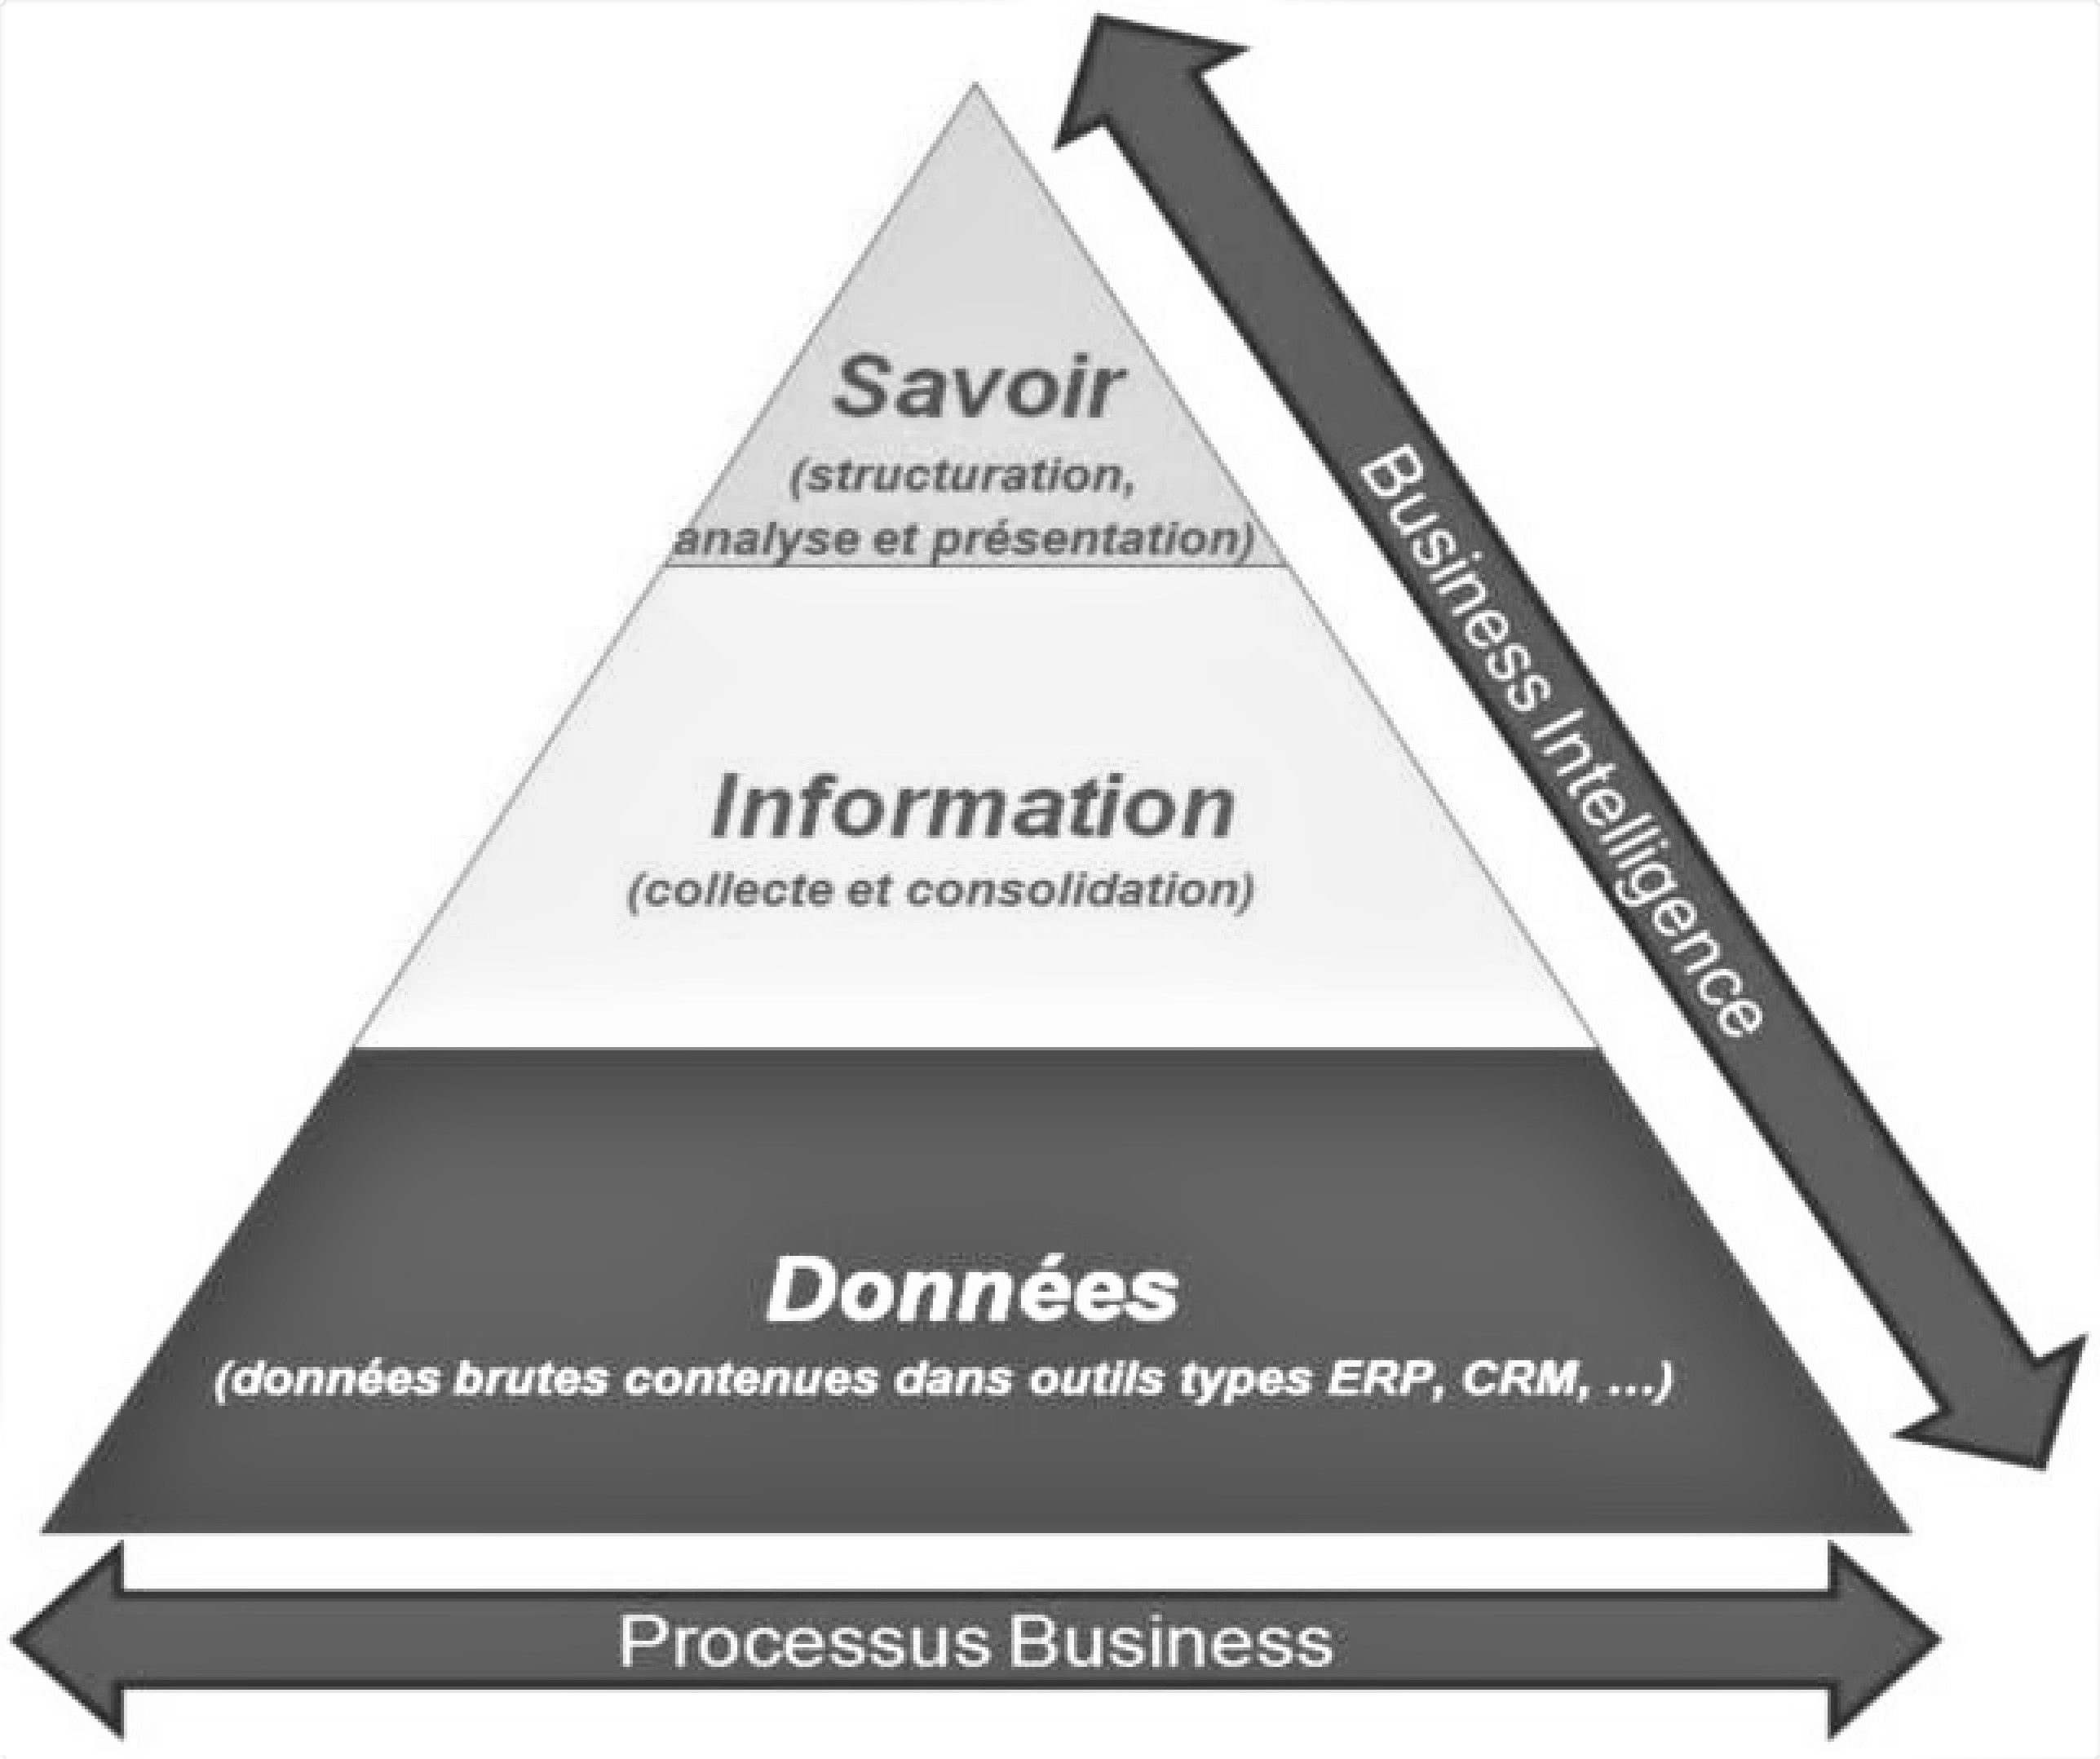
\includegraphics[width=100mm]{bi-image.jpg}
                \caption{ Pyramide modélisant le processus de la BI}
                \label{fig:pyramideBi}
            \end{figure}
            Il est coutumier de présenter les éléments et outils composant
            la chaîne décisionnelle en ses différentes parties, du cheminement
            depuis la donnée brute provenant du \acrlong{si} (\acrshort{si})
            sources(ERP, CRM...), à la production de reportings et autres tableaux
            de bord. Pour ce faire le schéma ci-dessous illustre :

    \section[Cadre théorique]{Cadre théorique}
        \subsection[Le Processus Unifié (UP)]{Le Processus Unifié (\acrshort{up})}
            \subsubsection[Définition]{Définition}    
            Le Processus Unifié (ou \acrshort{up}, \acrlong{up} en anglais) est un
            processus de développement logiciel \enquote{itératif et incrémental,
            centré sur l’architecture, conduit par les cas d’utilisation
            et piloté par les risques}. \cite*{Roques2008} Le processus unifie
            est constitué d’un ensemble de directive qui permettent de produire
            un logiciel à partir des exigences et des besoins des utilisateurs.
            \subsubsection[Caractéristiques du processus unifié]{Caractéristiques du processus unifié}
            Le processus unifié est une méthode de développement de logiciel caractérisée par :
            \par
            \begin{itemize}
                \setlength{\itemsep}{0pt}
                \item [\ding{226}] \textbf{Un pilotage par les cas d’utilisation} : le projet est mené en
                tenant compte des besoins et des exigences des utilisateurs. Les cas d’utilisation du
                futur système sont identifiés, décrits avec précision et priorisés.
                \item [\ding{226}] \textbf{Une démarche centrée sur l’architecture} : tout système
                complexe doit être décomposé en parties modulaires afin de garantir une maintenance et une
                évolution facilitées. Cette architecture (fonctionnelle, logique, matérielle, etc.)
                doit être modélisée en UML et pas seulement documentée en texte.
                \item [\ding{226}] \textbf{Une approche itérative et incrémentale} : Il est itératif en ce
                sens que chaque itération est réalisée avec les mêmes activités. À l’issue de chaque itération,
                une livraison partielle de l’itération est évaluée.
                \par\noindent
                Ainsi, un projet est divisé en une suite d’itérations. Chaque itération est une brique
                ajoutée à l’itération précédente qui doit donc avoir été préalablement réalisée.
                Quand la dernière itération est réalisée, c’est le projet dans son intégralité qui
                est alors achevé.
            \end{itemize}
            \begin{figure}[H]
                \centering
                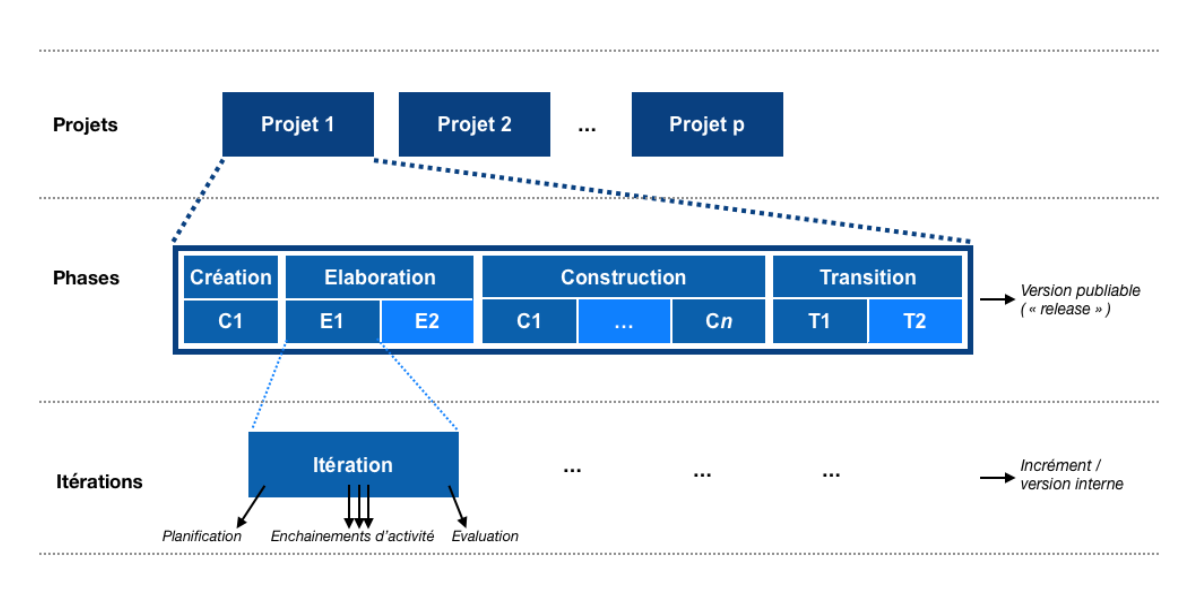
\includegraphics[width=130mm]{Cycle_de_dévelopement_du_processus_unifié.png}
                \caption{Diagramme illustrant le cycle de développement :
                projets, phases et itérations}
                \label{fig:CycleDeDev}
            \end{figure}
            Le processus unifié, organisé en fonction du temps, est divisé en quatre phases
            successives. \cite{gabay2008uml} :
            \par
            \begin{enumerate}
                \setlength{\itemsep}{0pt}
                \item \textbf{La phase d'inception} : Cette phase correspond à l’initialisation du
                projet où l’on mène une étude d’opportunité et de faisabilité du système
                à construire. Une évaluation des risques est aussi réalisée dès cette phase.
                \item \textbf{La phase d’élaboration} : Cette phase reprend les résultats de
                la phase d'inception et élargit l’appréciation de la faisabilité sur la quasi-totalité
                des cas d’utilisation. Ces cas d’utilisation se retrouvent dans le diagramme
                des cas d’utilisation qui est ainsi complété.
                \item \textbf{La phase de construction} : Cette phase correspond à la production
                d’une première version du produit. Elle est donc fortement centrée sur les activités
                de conception, d’implémentation et de test. En effet, les composants et
                fonctionnalités non implémentés dans la phase précédente le sont ici.
                \item \textbf{La phase de transition} : la phase de transition permet de faire
                passer le système informatique des mains des développeurs à celles des utilisateurs finaux.
                Les mots-clés sont : conversion des données, formation des utilisateurs,
                déploiement, béta-tests. \cite{Roques2008}
            \end{enumerate}
            \begin{figure}[H]
                \centering
                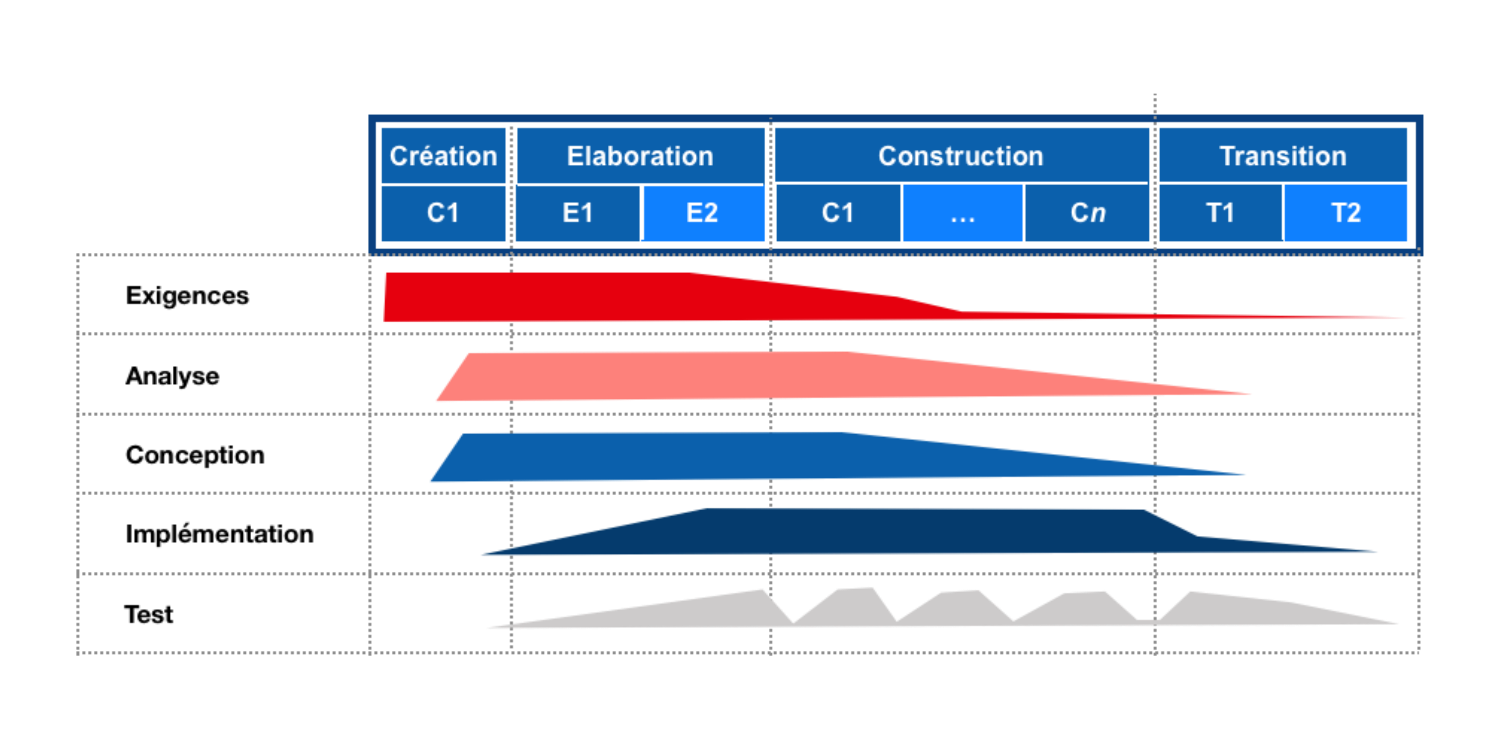
\includegraphics[width=130mm]{Processus_unifié_-_enchainements_d'activités_au_cours_du_cycle_de_vie.png}
                \caption{Diagramme illustrant l’évolution de l’importance
                relative des différentes disciplines au cours du projet}
                \label{fig:UpsProfil}
            \end{figure}
            
            \subsubsection[Démarche UP centrée sur l’architecture]{Démarche UP centrée sur l’architecture}
            Une architecture adaptée est la clé de voûte du succès d’un développement. Elle décrit
            des choix stratégiques qui déterminent en grande partie les qualités du logiciel (adaptabilité,
            performances, fiabilité...). \cite{diga2001uml}
            il existe des digrammes nécessaires à modéliser pour la réalisation d’un processus unifié.
            \par
            UML est constitué de 13 diagrammes officiels qui représentent chacun un concept du
            système ou du logiciel. Le logiciel peut être vu en considérant les aspects fonctionnels et
            les aspects d’architecture du logiciel. Ces deux aspects sont composés de cinq vues du
            logiciel à développer, organisés autour des besoins des utilisateurs.
            \par            
            Voici les cinq vues regroupant, uniquement, les différents diagrammes que nous
            utiliseront dans notre travail :
            \begin{enumerate}
                \setlength{\itemsep}{0pt}
                \item \textbf{La vue des besoins utilisateurs} est celle qui guide toutes les autres.
                Elle définit les besoins des clients du système et centre la définition de
                l’architecture du système sur la satisfaction (la réalisation) de ces besoins. \cite{diga2001uml}
                Cette vue comprend :
                \par
                \begin{dinglist}{226}
                    \setlength{\itemsep}{0pt}
                    \item Le diagramme de cas d’utilisation représente les fonctionnalités (autrement
                    dit cas d’utilisation) nécessaires aux utilisateurs.
                \end{dinglist}
                \item \textbf{La vue du processus}  démontre la décomposition du système en processus et en action ; les interactions
                entre les processus ainsi que la synchronisation et la communication des activités
                parallèles. Elle comprend :
                \par
                \begin{dinglist}{226}
                    \setlength{\itemsep}{0pt}
                    \item Le diagramme de séquence qui permet de décrire les différents scénarios
                    d’utilisation du système.
                    \item Le diagramme d’activité qui représente le déroulement des actions, sans utiliser
                    les objets. En phase d’analyse, il est utilisé pour consolider les spécifications d’un
                    cas d’utilisation.
                \end{dinglist}
                \item \textbf{La vue logique} a pour but d’identifier les éléments du domaine, les relations et
                interactions entre ces éléments. Elle comprend :
                \par
                \begin{dinglist}{226}
                    \setlength{\itemsep}{0pt}
                    \item Le diagramme de classes qui représente les entités
                    (des informations) manipulées par les utilisateurs, dans la phase d’analyse.
                \end{dinglist}
                \item \textbf{La vue des composants} met en évidence les différentes parties qui
                composeront le futur système (fichiers sources, bibliothèques, bases de données,
                exécutables, etc.). Elle comprend :
                \par
                \begin{dinglist}{226}
                    \setlength{\itemsep}{0pt}
                    \item Le diagramme de composants qui décrit tous les
                    composants utiles à l’exécution du système (applications, librairies,
                    instances de base de données, exécutables, etc.).
                \end{dinglist}
                \par
                \item \textbf{La vue de déploiement} décrit les ressources matérielles et la répartition des parties du
                logiciel sur ces éléments. Elle ne comprend qu’un seul diagramme qui est :
                \par
                \begin{dinglist}{226}
                    \item Le diagramme de déploiement qui correspond à la description de l’environnement
                    d’exécution du système (matériel, réseau…) et de la façon dont les composants y sont
                    installés.
                \end{dinglist}
            \end{enumerate}

        \subsection[La méthode GIMSI]{La méthode \acrshort{gimsi}}
            \subsubsection[Définition]{Définition}
            \acrshort*{gimsi} est une méthode de conception du système de pilotage à base 
            de tableaux de bord, centrée sur les femmes et les hommes,
            tous décideurs confrontés au risque et à la complexité. \cite*{fernandez2021gimsi} Elle
            peut aussi être défini comme une méthode de conception et de réalisation de
            système décisionnel en entreprise.
            \par
            GIMSI est l’acronyme de :
            \par
            \begin{itemize}
                \setlength{\itemsep}{0pt}
                \item [\ding{226}] \textbf{G} comme Généralisation :
                la méthode s’utilise dans différents domaines.
                \item [\ding{226}] \textbf{I} comme Information : l’accès à l’information
                pertinente est le fondement de l’aide à la décision.
                \item [\ding{226}] \textbf{M} comme Méthode et Mesure : c’est une méthode
                et la mesure en est le principe.
                \item [\ding{226}] \textbf{S} comme Système et Systémique : son but est de construire le système de pilotage
                et de l’intégrer au cœur du système d’information.
                \item [\ding{226}] \textbf{I} comme Individualité et Initiative : cette méthode privilégie
                l’autonomie des individus pour une prise d’initiative plus naturelle.
            \end{itemize}
            \subsubsection[Démarche de conception et de réalisation]{Démarche de conception et de réalisation}
            La méthode GIMSI est structurée selon 10 étapes
            bien identifiées et classées en quatre phases thématiques qui sont présenté
            dans \cite*[Tab. \ref{table:phaseEtapeGimsi}]{fernandez2011nouveaux} :
            \begin{longtable}{p{3cm} p{0cm} p{4cm} p{5cm}}
                \caption{Phases et étapes de GIMSI}
                \label{table:phaseEtapeGimsi}
                \\\hline\hline
                    \textbf{Phases} & \textbf{N} & \textbf{Étapes} & \textbf{Objectif}
                \\\hline\hline
                    \textbf{Identification} & 1 & Environnement
                    de l’entreprise & Analyse de l’environnement économique
                    et de la stratégie de l’entreprise afin de
                    définir le périmètre et la portée du projet
                    \\
                        & 2 & Identification de l’entreprise & Analyse des structures
                    de l’entreprise pour identifier les processus, activités et acteurs concernés
                    \\
                    \textbf{Conception} & 3 & Définition des objectifs & 
                    Sélection des objectifs tactiques de chaque équipe
                    \\
                        & 4 & Construction du tableau de bord & Définition du tableau
                    de bord de chaque équipe
                    \\
                        & 5 & Choix des indicateurs & Choix des indicateurs en fonction
                    des objectifs choisis
                    \\
                        & 6 & Collecte des informations & Identification des informations nécessaires
                    à la construction des indicateurs
                    \\
                        & 7 & Le système de tableau de bord & Construction du
                    système de tableaux de bord, contrôle de la cohérence globale
                    \\
                    \textbf{Mise en œuvre} & 8 & Le choix des progiciels &
                    Élaboration de la grille de sélection pour le choix des progiciels adéquats
                    \\
                    & 9 & Intégration et déploiement & Implantation des progiciels,
                    déploiement à l’entreprise
                    \\
                    \textbf{Amélioration permanente} & 10 & Audit & Suivi
                    permanent du système
                \\\bottomrule
            \end{longtable}
    \section[Conclusion partielle]{Conclusion partielle}
    Dans ce chapitre, nous avons parlé de deux grands points qui sont : le cadre conceptuel
    et le cadre théorique. Pour ce qui est du cadre conceptuel nous avons défini
    les concepts clés que nous retrouverons dans l’application et pour ce qui est du cadre théorique,
    nous avons parlé des théories liées au processus UP et à la méthode GIMSI. 